Now we need to find a way to quantify risk, especially systemic risk (idiosyncratic risk can be diversified away), of an asset or an asset in our portfolio. 

\begin{multicols}{2}
    
In the CAPM framework, all investors are assumed to have access to the same information and hold homogeneous expectations about future returns, and the market portfolio is considered to be the only efficient portfolio, meaning that it offers the highest expected return for a given level of risk.\par 

Then we can effectively transfer our original Tangency Portfolio into our \underline{\textbf{Market portfolio}}, and our capital allocation line (CAL) into \underline{\textbf{Capital Market Line}}, the line that connects the Market Portfolio to the risk-free rate
\begin{figure}[H]
    \centering 
    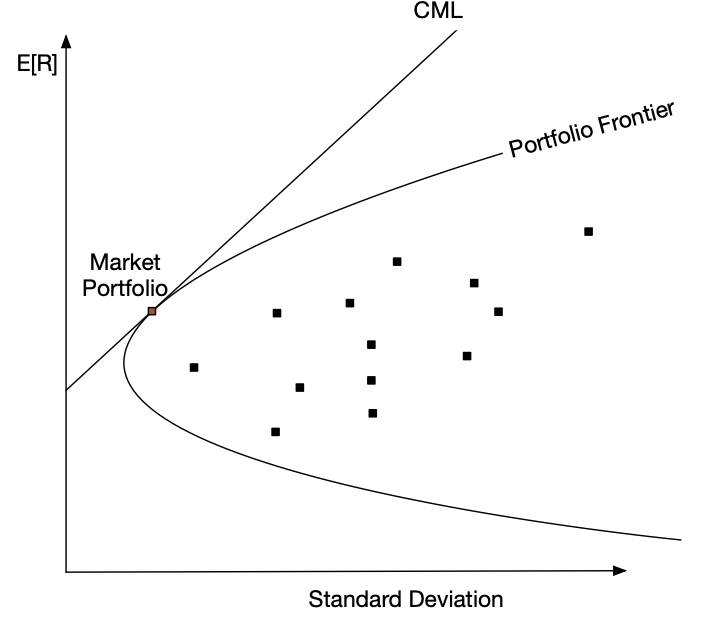
\includegraphics[width =0.4\textwidth]{Figure/cml.png}
\end{figure}
Given the assumption, the risk-reward ratio of any asset or portfolio is determined solely by its beta, and the expected return for each unit of systematic risk should be the same for all assets and portfolios. 
\begin{gather*}
    \frac{E[R_i]-R_f}{Cov[R_M, R_i]} = \frac{E[R_M]-R_f}{V[R_M]}\\[0.1cm]
    E[R_i] = (E[R_M]-R_f)\frac{Cov(R_M,R_i)}{V[R_M]}+R_f\\
    \boxed{E[R_i] =  R_f + \beta(E[R_M]-R_f)}
\end{gather*}
$\beta$ is therefore the measure of systemic risk of an asset. This is because according to CAPM in an efficient market, investors are only compensated for bearing systematic risk, which is the risk that cannot be diversified away by holding a diversified portfolio.

The amount that an investor allocates to the market portfolio is negatively related to \underline{\textbf{(1)}} the investor's risk aversion coefficient, \underline{\textbf{(2)}} the risk-free rate of return, \underline{\textbf{(3)}} the variance of the market portfolio.

\subsection{Application of CAPM (1) -- Excess Return}
Analyst compare stocks' returns with their fair expected return from the CAPM
\begin{gather*}
    \alpha = E[R_i]-[R_f+\beta(E[R_M]-R_f)]
\end{gather*}
A stock's $\alpha$ is the unexpected deviation from the fair return. Stocks with high alpha are under-valued and should be bought.

\subsection{Application of CAPM (2) -- Capital Budgeting Decisions}
CAPM can also be used to judge whether firms should undertake risky projects. This can be done by calculating the Net Present Value (NPV) or compare the CAPM expected return with internal rate of return (IRR) (the rate of return where NPV = 0). If $E[R_i]>IRR$, then the firm should reject the project. 

\subsection{Index Model}
An index model uses an actual stock index to proxy this theoretical market. CAPM makes forward-looking predictions. Index models use historical data. Index model states that
\begin{gather*}
    R_i-R_f = \alpha_i+\beta_i[R_M-R_f]+\varepsilon_i
\end{gather*} 
$\alpha$ is the abnormal return and $\varepsilon$ is the firm specific risk, which is idiosyncratic risk. And the CAPM equation can be rewritten in terms of the index model
\begin{gather*}
    \boxed{R_i = R_f+\beta_i[R_M-R_f]+\varepsilon_i}
\end{gather*}
The variance percentage of the idiosyncratic risk and systemic risk can therefore be quantify as 
\begin{gather*}
    \begin{split}
        V[R_i] &= V[R_f+\beta_i[R_M-R_f]+\varepsilon_i]\\
        \sigma_i^2 &= V[\beta_i(R_M-R_i)+\varepsilon_i]\\
        &= \beta_i\sigma_M^2 + \bar{\sigma_i}^2
    \end{split}
\end{gather*}
$\boxed{\bar{\sigma_i}^2/\sigma_i^2}$ is the variance percentage that is \textbf{idiosyncratic} and 1-term will then be the systemic risk








\end{multicols}